\chapter{Methodology}
This chapter covers the various methodologies that were implemented in this project, this includes Research methodologies, Software development methodologies, project management, supervisor meetings, developments tools, testing and source control.\newline

An overview of methodologies used in this project; \textbf{Research methodologies} which includes Mixed Methods, Quantitative Research and Qualitative Research.
\textbf{Software development methodologies} which includes Agile Development, Continuous Delivery, Test Driven Development, Feature Driven Development, Extreme Programming etc.
\textbf{Project management} which includes GitHub Kanban board and supervisor meetings.
\textbf{Development tools} Android studio, Firebase.
\textbf{Source Control} GitHub, Overleaf, Badge/Shield

\newpage

\section{Research Methodology}
The research methodology that was used in this project was a Mixed Methods 
Research methodology, using a mix of both Qualitative Research and Quantitative 
Research. Qualitative research approaches are employed across many academic 
disciplines and is useful at an individual level. Qualitative data collection
methods vary using unstructured or semi-structured techniques.

\medskip
Various data collection tools were used for gathering data such as

\section{Project management}
\begin{center}
    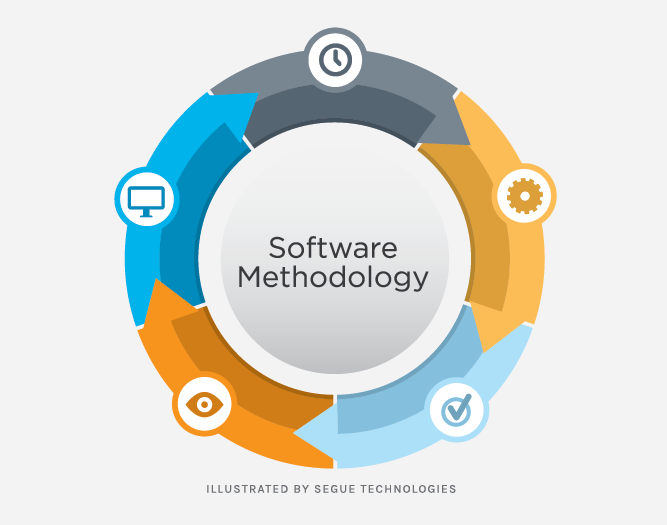
\includegraphics[width=8cm,keepaspectratio]{Images/Software_Method.png}

\end{center}
\par
\par
\medskip
Project Management is a key element of any task to ensure that the project is laid out correctly and each component party is complete at a given date. Because this project is a solo project i used the GitHub Kanban board to first pick features that i may want to implement and then broke them down into separate cards that i could work on individually. This helped brake down tasks which helped in development.

\subsection{Agile}
This project used Agile project management methodologies. An iterative approach was taken. This meant that each week i had certain tasks laid out to be completed be that either a feature for the app or documentation. I also had short weekly/bi-weekly meetings with my supervisor where i would update him, and asks for advice on my dissertation, app, etc. 

\subsubsection{Agile Road-map}
An agile road-map in agile development helps state the goals of the project from the outset. It helps break down the tasks which are then further broken down for sprints. This is usually a high level view of the project. It is used often in industry and it helps to understand a project as a whole and learn what other teams are contributing to the overall project. The roadmap also shows how the project can grow in the future.

\subsubsection{Planning and Development}
During the meeting and planning phase, the milestones \& objectives for the project were identified and broken down into simpler, and more manageable tasks. The tasks are were then grouped into sprints or iterations lasting one to three weeks depending on the task. These are the tasks which mostly completed before each meeting with my supervisor. With each meeting i had a task somewhat completed and i could then know the following task which i could talk with my supervisor about before hand. So each weekly meeting with the supervisor started a sprint and the aim was to complete most of that sprint before the next meeting. The plans for the project and the sprints are taken from the User stories i created on the Kanban project and Design document. Through this iteration i convert the plans into working code.

\subsubsection{Design Phase}
Throughout the agile development life cycle design is a step in every iteration/sprint. The design is gradually built on. The design is never defined at the beginning of the project. The gradual evolution of the design enables taking advantages of new technologies that come on stream as well as meeting any new requirements brought forward by clients. The user experience is key when design a project/application. Every design must be user friendly. The type of end user of the item must be consider when designing. This comes to play in android development often as there is many different tools in development to create different features. You need to test them to know whats best for the end product.

\subsubsection{Testing}
Testing was carried out continuously with Android Studio features. Not only those Android Studio have a huge amount of features the Emulator can test a massive array of devices. So testing for this application was a continuous process throughout every build.

In a real-world environment The user tests would be carried out when meeting with the client. The client using the application would then comment on any changes that should be or could be made.

\section{System Integration}

\subsection{Test Driven Development}
\subsection{Feature Driven Development}
\subsection{Continuous Delivery}
\subsection{Extreme Programming}

\section{Development tools}
In order to manage this project i used different development tools and Source Control tools. This was very useful as it enables working on different branches for features that i want to implement and leaves the master branch as a working state of the project. This could be used for industry standard as continuous delivery. For this project it's meant that after each sprint there was a working version to present to the customer. Although the working version does not mean it doesn't need changes in next sprints. I was solo this project so i did not take advantage of branches as much as a group would, as each member would have there own branch to work on.

\subsection{Android Studio}
Android Studio is the official integrated development environment (IDE) for Google's Android operating system, built on JetBrains' IntelliJ IDEA software and designed specifically for Android development. It is available for download on Windows, macOS and Linux based operating systems.It is a replacement for the Eclipse Android Development Tools (ADT) as the primary IDE for native Android application development.\newline

The integration between Android Studio and Firebase made Android Studio the most superior development platform to use.

\subsection{Firebase}
Firebase  is  Google’s  mobile  and  web  application  development  platform  that helps you build,  improve,  and grow your application.  Firebase frees developers to focus on crafting excellent user experiences.  You don’t need to manage servers.  You don’t need to write APIs.  Firebase is your server, your API and your database, everything is written generically so that you can modify every-thing  to  suit  most  needs.   

\section{Source Control}

\subsection{GitHub}
Github provides hosting for software development version control using Git. It offers the distributed version control and source code management (SCM) functionality of Git, plus its own features. It provides access control and several collaboration features such as bug tracking, feature requests, task management, and wikis for every project. GitHub offers plans free of charge, and professional and enterprise accounts. The Github kanban board was a feature i used in this project to track sprints.

\subsection{Overleaf}
Overleaf is an open-source online real-time collaborate LaTeX editor. It is hosted at http://www.overleaf.com, but can also run on your own local version, and contribute to the development of Overleaf.
\subsection{Badge/Shield}
Badge/Shield.io is a service for concise, consistent, and legible badges in SVG and raster format, which can easily be included in GitHub READMEs or any other web page. The service supports dozens of continuous integration services, package registries, distributions, app stores, social networks, code coverage services, and code analysis services. Every month it serves over 470 million images.
This is used for easy access to a copy of the APK and Dissertation at the top of my README, you can further customize these badges to show Beta versions, stable versions, downloads, ratings, code coverage etc.

